#\section{Holdback Queue}

Die Holdback Queue enthält alle Nachrichten, die nicht ausgeliefert werden dürfen. Das heißt, dass die enthaltenen Nachrichten nicht die richtigen Nummern haben für die Delivery Queue haben. Durch regelmäßiges Prüfen wird entschieden, ob inzwischen eine geeignete Nachricht für die Delivery Queue von den Redakteuren empfangen wurde. 

Da die Nachrichten nach aufsteigender Nummerierung an die Delivery Queue weitergeleitet werden, bietet es sich an diese in der Holdback Queue bereits zu sortieren. 
Um diese Sortierung möglichst effizient zu gestalten werden verschiedene Algorithmen getestet (siehe Kapitel \ref{Problemstellungen}.).

Die Holdback Queue kann in zwei möglichen Strukturen verwaltet werden. Da nach jedem Einfügen das Element in die Queue "reinsortiert" werden muss, wäre es zum einen möglich, das Element vorne in die Queue einzufügen und dann über den InsertionSort Algorithmus zu sortieren. Dies würde einen linearen Aufwand also $O(n)$ bedeuten, da jedes Element mit jedem Element verglichen werden muss. Im Schnitt wäre es möglicherweise sogar $O(n/2)$, da das Element nicht unbedingt immer am Ende der Queue stehen muss. 
Die zweite Möglichkeit wäre der Aufbau der Queue in Form eines HeapSorts. Der HeapSort Algorithmus an sich setzt eine Komplexität von $O(n*log(n))$ voraus. Das liegt aber daran, dass dieser zuerst zu einem Heap umstrukturiert werden muss. Da dieser Schritt aber entfällt, angenommen man strukturiert diesen Heap von Anfang an, dann bleibt eine Komplexität von $O(log(n)$. Da das kleinste Element genauso oft gefragt ist wie das größte Element, spielt es für die Laufzeit keine Rollte, ob das größte Element die Wurzel des Heaps ist oder das kleinste. Somit kann theoretisch einfach der HeapSort Algorithmus aus der vorherigen Praktikumsaufgabe übernommen werden. 
Für die Struktur des HeapSorts gilt, dass jedes Element die Form {[}Nnr, Msg, TSclientout{]}, Höhe, linkerTeilbaum, rechterTeilbaum] hat. Außerdem ist die Nnr des Wurzelelements stets größer als die der Kinderelemente. Die beiden Kinderelemente werden nicht miteinander verglichen. 
Für das Einfügen eines neuen Elements entsteht dadurch der Vorteil, dass das Element im Normalfall nicht durch den Heap versickern muss, da es die größte Nachrichtennummer haben sollte und somit ganz oben als Wurzel eingefügt wird. Es ensteht für diesen Prozess eine Komplexität von $O(1)$. Beim Entfernen eines Elements muss nun allerdings das letzte also kleinste Element gesucht werden. Das wäre in diesem Falle das Element mit dem größten Index, also bildlich gesehen das Element unten rechts im Heap. 
//TODO Korrektur Für die Struktur des HeapSorts gilt, dass jedes Element die Form {[}Nnr, Msg, TSclientout{]}, Höhe, linkerTeilbaum, rechterTeilbaum] hat. Außerdem ist die Nnr des Wurzelelements stets kleiner als die der Kinderelemente. Die beiden Kinderelemente werden nicht miteinander verglichen. Diese Form des Heaps nennt sich Min Heap. 
Für das Entfernen eines neuen Elements entsteht dadurch der Vorteil, dass das Element im Normalfall die Wurzel des Heaps ist, da es die kleinste Nachrichtennummer haben sollte und somit ganz oben als Wurzel gespeichert ist. Es entsteht für diesen Prozess eine Komplexität von $O(1)$. Auch beim Einfügen des Elements ist der Heap von Vorteil, da die Elemente ohne erkennbare Sortierung in den Heap eingefügt werden (siehe \ref{fig:HBQFilesEntry}). Die Elemente werden als Wurzel eingefügt und versickern dann im Heap bis sie ihre Position erreicht haben. Es entsteht eine Komplexität von $O(log(n))$. Wenn der Durchschnitt betrachtet wird kommt es sogar zu $O(log(n)/2)$, da die Elemente nicht immer bis ans Ende des Heaps sortiert werden, sondern genauso gut an den Anfang kommen können.

\begin{figure}[htbp]
\begin{center}
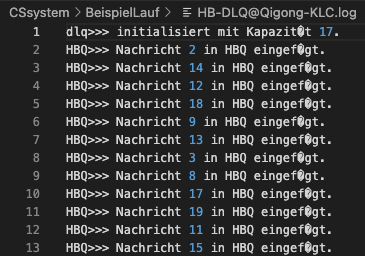
\includegraphics[scale=0.6]{Bilder/HBQFilesEntry.png}
\caption{\label{fig:HBQFilesEntry} Nachrichtendienst \cite{HBQlogging}} 
\end{center}
\end{figure}

\subsection{Operationen}

\subsubsection{initHBQ}

Beim Initialisieren der Holdback Queue liegt das größte Problem darin, die Queue auf einem Node zu speichern. Dies geschieht durch den Aufruf spawn(). Hierbei wird ein neuer Prozess erzeugt und Initialisiert. Die ProzessID dieses neu erzeugten Prozesses wird als Rückgabewert zurückgegeben und in einer Variable gespeichert. 
Die lokale Registrierung des Prozesses findet über den Aufruf register() statt. Als Parameter werden hier einmal die ProzessID des zu registrierenden Prozesses übergeben und das Atom unter welchem dieser Prozess lokal gespeichert werden soll. 
Außerdem wird die Initialisierung der Delivery Queue auch über die Holdback Queue aufgerufen. Diesem Aufruf wird der Parameter DLQ-Limit mit übergeben. 

Umsetzung der Nebenläufigkeit in Erlang. Durch Rekursion kann der Status des Prozesses, also in diesem Falle der Inhalt der Holdback Queue, die Delivery Queue, die in die zu loggende Datei und der aktuell nächste leere Index, vollständig in den Parametern der Funktion gehalten werden \cite{learnErlang}. Der Prozess der Holdback Queue wird hierfür über die Funktion loop gestartet. Dieser Funktion wird als Parameter die Holdback Queue übergeben und somit kann diese über jeden loop Aufruf beschrieben und gelesen werden. 

\subsection{checkHBQ}

Da die Nachrichten der Holdback Queue regelmäßig auf Auslieferbarkeit geprüft werden sollen, wurde hierfür eine weitere Funktion implementiert. 
In dieser wird das derzeitige erste Element der Holdback Queue (im Folgenden "SmallestElem")  mit der von der Delivery Queue erwarteten Nummer ("ExpNrDLQ") verglichen. 
Somit kann erkannt werden, ob Elemente aus der Holdback Queue verworfen oder an die Delivery Queue ausgeliefert werden sollen. 
Wenn zum Beispiel SmallestElem == ExpNrDLQ gilt, dann wird SmallestElem an die Delivery Queue ausgeliefert. Im Falle SmallestElem < ExpNrDLQ wird das SmallestElem verworfen, da es nicht mehr benötigt wird und ansonsten die Holdback Queue nur unnötig blockieren würde. Benötigt wird es nicht mehr, da die Delivery Queue als \( $dlq(n)$ = \sum \limits_{i=1}^n i\)
definiert ist. Wenn also i = n ist, dann werden alle Elemente kleiner n von der Delivery Queue nicht mehr angefragt und können somit aus der Holdback Queue verworfen werden.  
Für den Fall, dass die Holdback Queue keine Elemente mehr enthält wird eine entsprechende Ausgabe geloggt. 

Die Funktion wird nach jeder Ausführung der pushHBQ Funktion aufgerufen. Somit ist sichergestellt, dass nach jeder Veränderung der Queue einmal geprüft wird, ob diese noch synchronisiert ist und keine unnötigen Elemente enthält. 

\subsubsection{pushHBQ} 

In dieser Funktion wird eine Nachricht in die Queue geschrieben. Die Nachricht enthält die entsprechende Nachrichtennummer, den Inhalt der Nachricht und einen Timestamp, wann der Client die Nachricht abgeschickt, bzw. die Holdback Queue diese empfangen hat. Wie bereits oben beschrieben wird, bedingt durch die fehlende Sortierung der Clients, jedes Element oben als Wurzel eingefügt und dann nach unten versickert. Hierbei gilt, solange linkerTeilbaum \textgreater Wurzelelement dann Wurzelelement $\rightarrow$ linkerTeilbaum und linkerTeilbaum $\rightarrow$ Wurzelknoten.
 
Zum Bestimmen der Position wird wie in der letzten Praktikumsaufgabe die sortv.erl Datei verwendet. Hier wird als Parameter die Position, also der höchste freie Index mit übergeben. Dieser muss also bei jedem Einfügen eines Elements erhöht und beim Löschen eines Elements um eins verkleinert werden. 
Aus der zurückgegebenen Liste kann der Pfad bestimmt werden, an welchem das letzte Element eingefügt werden soll. So kann zum Beispiel eine Liste mit den Elementen {r,l,r,r} zurückgegeben werden. Diese beschreibt den von oben versickernden Pfad für den letzten freien Index.
Die Position des höchsten Index wird als Integer zusammen mit der Holdback Queue als Parameter in der loop Funktion mit übergeben und somit rekursiv gespeichert. 

Da in der Delivery Queue nur eine bestimmte Anzahl an Nachrichten stehen kann, wird bei der Holdback Queue ab einer erreichten Größe von $2/3\;*\;sizeOfDLQ$ versucht der Inhalt der Queue zu reduzieren. Dafür wird geprüft, ob eine Lücke zwischen den beiden Queues entstanden ist. Ein Beispiel dafür ist in Abbildung \ref{fig:BeispielHBQFehler} zu sehen. Hier hat die Holdback Queue eine bestimmte Größe erreicht und die Lücke in der Delivery Queue wird dementsprechend aufgefüllt. Die Fehlermeldung wird in Textform in die Delivery Queue eingetragen.

Die Elemente welche aus der Holdback Queue an die Delivery Queue gesendet wurden, müssen aus der Holdback Queue gelöscht werden, da ansonsten ihre Größe nicht berechnet werden kann. 
Dies geschieht, da beim Einfügen immer das kleinste Element aus der Holdback Queue mit der von der Delivery Queue erwarteten Nummer verglichen wird. Das kleinste Element der HBQ ist dessen Wurzelelement. Dieses muss größer gleich der erwarteten Nummer sein. 
Ansonsten kommt es zu einem Ausnahmefall, welcher aber bedingt durch das Verwerfen von Nachrichten, welche kleiner als die erwartete Nummer sind, eigentlich nicht vorkommen dürfte. Zur Sicherheit wird in dieser Funktion die Holdback Queue ansonsten synchronisiert, das heißt, dass das Wurzelelement solange gelöscht wird, bis dieses größer gleich dem erwartetem Element der Delivery Queue ist. 
Für den Fall das es größer ist, wird eine Fehlermeldung in die log Datei geschrieben. In dieser steht die Differenz der fehlenden Elemente. Wenn also zum Beispiel am Anfang alle Elemente > 3 in die Holdback Queue eingefügt worden, dann fehlen die Elemente 1, 2 und 3 zum Einfügen in die Delivery Queue. In der Fehlermeldung steht also "Fehlernachricht für Nachrichten 1 bis 3 generiert. Die 3 wird als extra Nachricht in die Delivery Queue eingefügt.

Ein weiteres Problem entsteht, wenn Elemente eingefügt werden, welche eine kleinere Nachrichtennummer haben als das zu erwartende nächste Element der Delivery Queue. In diesem Falle wird die einzufügenden Nachricht verworfen und es wird NNr<expNrDLQ ausgegeben.

\begin{figure}[htbp]
\begin{center}
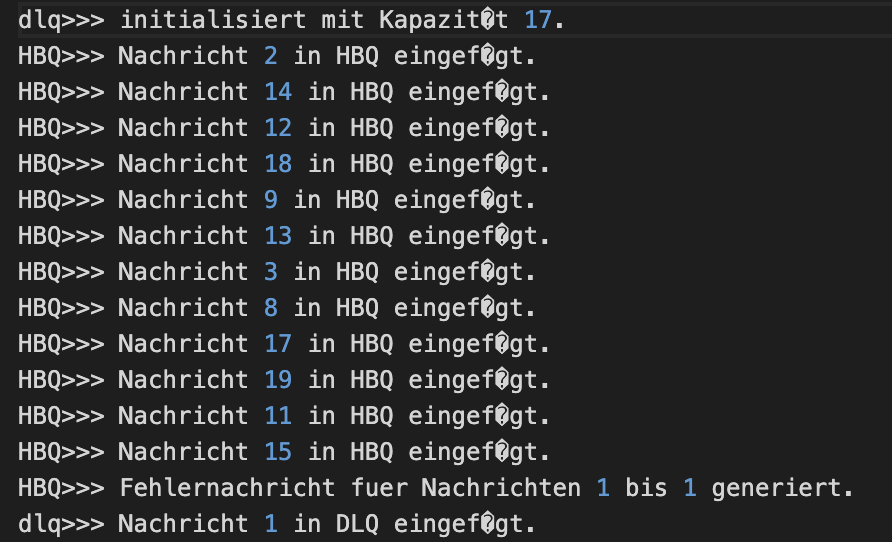
\includegraphics[scale=0.6]{Bilder/BeispielHBQFehler}
\caption{\label{fig:BeispielHBQFehler} Fehlermeldung Beispiel \cite{HBQfehler}} 
\end{center}
\end{figure}

\subsubsection{deliverMSG}

In dieser Funktion wird die Delivery Queue über die Holdback Queue beauftragt die zu der übergebenen Nachrichtennummer zugehörige Nachricht zu senden. Der Client welcher die Nachricht empfangen soll wird als ProzessID mit im Parameter der Funktion übergeben. 
Über den Funktionsaufruf dlq:deliverMSG(MSGNr, ClientPID, Queue, Datei) wird also die entsprechend zu sendende Nachrichtennummer, die ProzessID, die Delivery Queue und die in die zu loggende Datei übergeben. 
Wenn die übergebene Nachricht nicht verfügbar ist, dann wird die Nachricht mit der nächst größeren Nummer gesendet. 
Als Antwort von dem Prozess der Holdback Queue wird dann die gesendete Nachrichtennummer gesendet. 

\subsubsection{listADT}

Diese Funktion ist aufgeteilt in zwei verschiedene Funktionen: listHBQ und listDLQ. 
Es wird in beiden der Inhalt der jeweiligen Queue ausgegeben. Dabei wird die Reihenfolge der Queue beibehalten. Ausgegeben werden alle enthaltenden Nachrichtennummern in Form einer Liste. 

\paragraph{listHBQ}
Für diese Funktion kann über alle Elemente der Holdback Queue iteriert werden und jeweils die Nachrichtennummer in eine separate Liste geschrieben werden. 
Da die Holdback Queue hier in einer Heap Struktur umgesetzt ist, gibt es zwei mögliche Sortierungen. Zum einen könnte nach Index sortiert werden. Dementsprechend würde das Wurzelelement als erstes ausgegeben werden, dann alle Elemente mit der nächst kleinsten Höhe von links nach rechts gelesen usw..
Die andere Möglichkeit wäre es den Heap bei der Ausgabe zu sortieren. Es würde also das Wurzelelement als erstes ausgegeben werden, vor der nächsten Ausgabe wird dann aber erst der Heap neu strukturiert. Das Element mit dem höchsten Index wird die neue Wurzel. Dann versickert dieses so lange nach unten, bis es keinen kleineren Teilbaum mehr hat. Erst danach wird das nächste Element (also wieder die Wurzel) ausgegeben. 
Der Vorteil der Index-Sortierung ist die kleinere Laufzeit, da im Vergleich zur Nachrichtennummer-Sortierung nicht nach jeder Ausgabe neu strukturiert werden muss. Allerdings sind bei der Index-Sortierung die Nachrichtennummern in der Ausgabe zufällig, was z.B. das händische Finden eines Elements aufwändiger machen würde. 
Da die Funktionalität in diesem Falle im Vordergrund steht, wird bei listHBQ eine Liste in aufsteigend sortierter Reihenfolge ausgegeben. 

Die Ergebnisse werden in eine log Datei geschrieben und bei Erfolg wird als Rückgabewert ein ok als Antwort gesendet.

\paragraph{listDLQ}
Da es schon eine Funktion listDLQ für die Delivery Queue gibt, wird diese hier verwendet. 
Als Queue wird einfach die in der Holdback Queue gespeicherte DLQ übergeben und die zurückgegebene Liste wird dann in die Logging Datei geschrieben. 

\subsubsection{dellHBQ}

Um die HBQ zu löschen muss durch die rekursive Implementierung in die stetige Übergabe der Queue als Parameter, der Prozess beendet werden. Hierfür kann der von Erlang bereitgestellte Funktionsaufruf $exit(PID)$ verwendet werden. Nach diesem Aufruf sind dann weder die Elemente innerhalb der Queue noch vorhanden, noch ist die PID der Queue weiterhin referenziert. Falls das Terminieren fehlschlägt, wird eine Textnachricht $exiting_failed$ ausgegeben. 
Außerdem wird das Löschen der Delivery Queue von dieser Funktion initialisiert. 